\begin{figure}[ht]
    \centering
    % Subfigure 1
    \begin{subfigure}{0.32\textwidth}
        \centering
        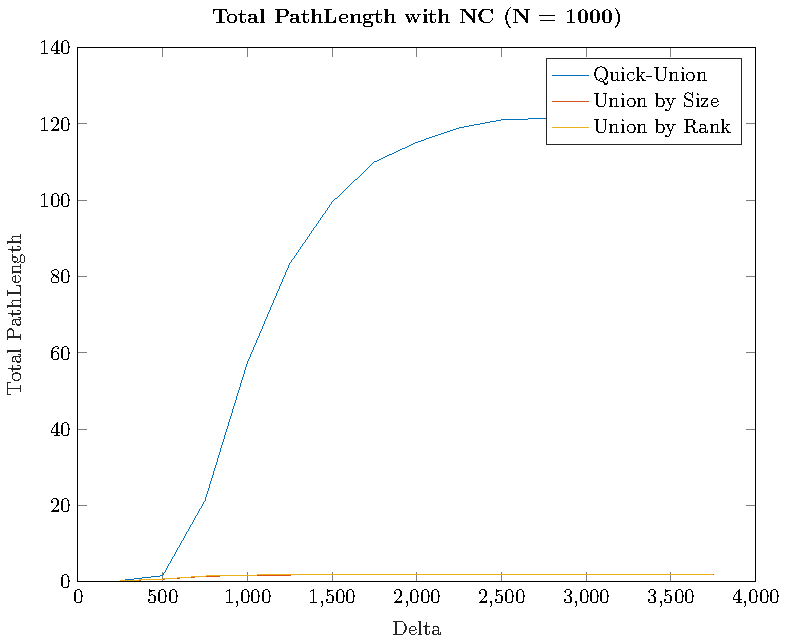
\includegraphics[width=\textwidth]{../images/plotNCFull1000_PathLength.pdf}
        \caption{Path Lengths with different union strategies with $n = 1000$}
    \end{subfigure}%
    \hfill
    % Subfigure 2
    \begin{subfigure}{0.32\textwidth}
        \centering
        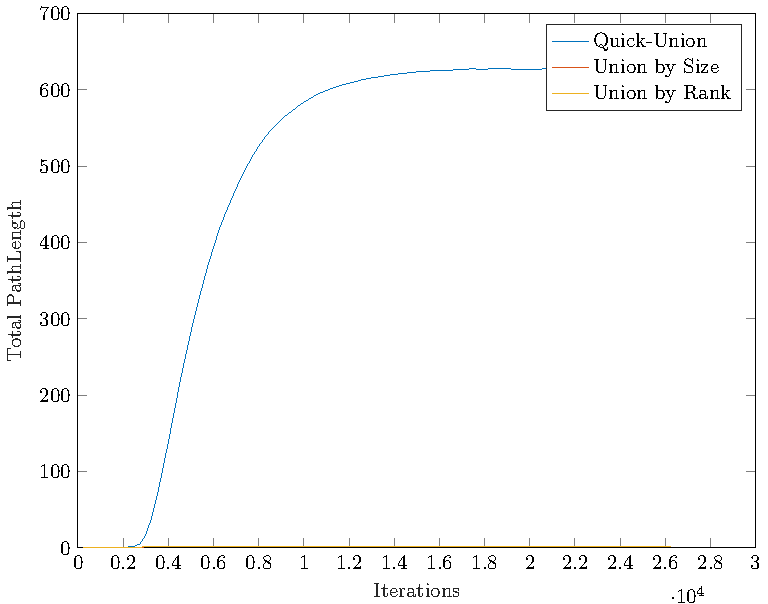
\includegraphics[width=\textwidth]{../images/plotNCFull5000_PathLength.pdf}
        \caption{Path Lengths with different union strategies with $n = 5000$}
    \end{subfigure}%
    \hfill
    % Subfigure 3
    \begin{subfigure}{0.32\textwidth}
        \centering
        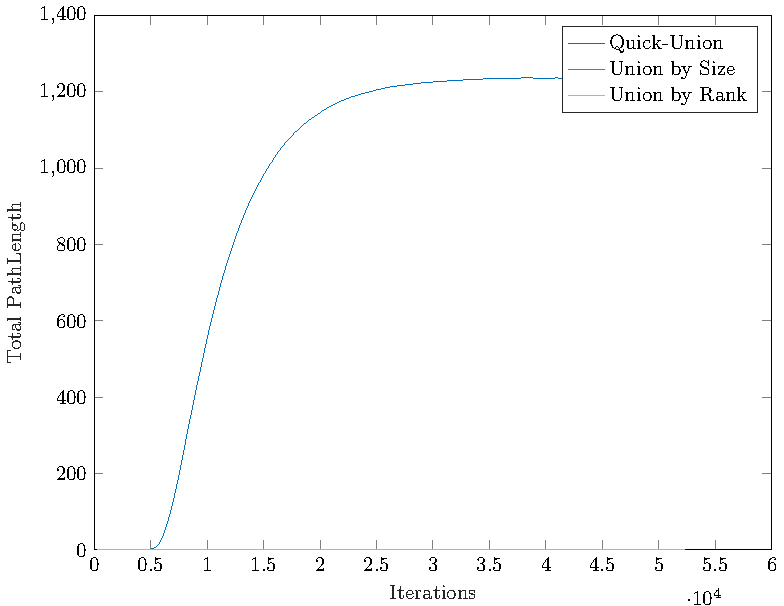
\includegraphics[width=\textwidth]{../images/plotNCFull10000_PathLength.pdf}
        \caption{Path Lengths with different union strategies with $n = 10000$}
    \end{subfigure}
    \begin{subfigure}{0.32\textwidth}
        \centering
        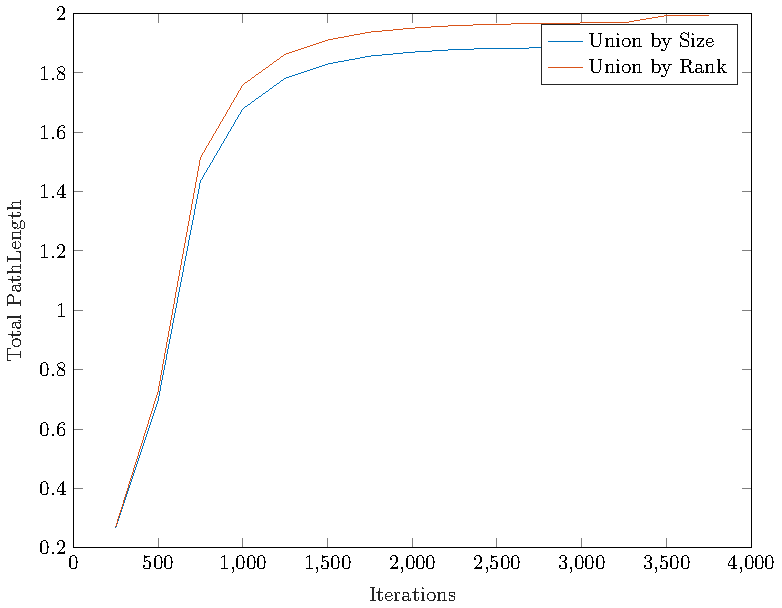
\includegraphics[width=\textwidth]{../images/plotNCNonFull1000_PathLength.pdf}
        \caption{Path Lengths with different union strategies with $n = 1000$ without Quick-Union}
    \end{subfigure}%
    \hfill
    % Subfigure 2
    \begin{subfigure}{0.32\textwidth}
        \centering
        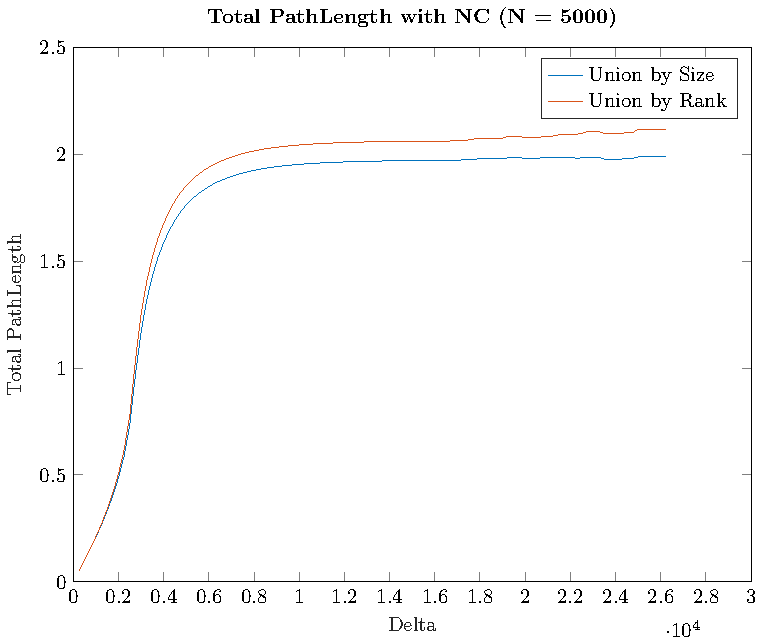
\includegraphics[width=\textwidth]{../images/plotNCNonFull5000_PathLength.pdf}
        \caption{Path Lengths with different union strategies with $n = 5000$ without Quick-Union}
    \end{subfigure}%
    \hfill
    % Subfigure 3
    \begin{subfigure}{0.32\textwidth}
        \centering
        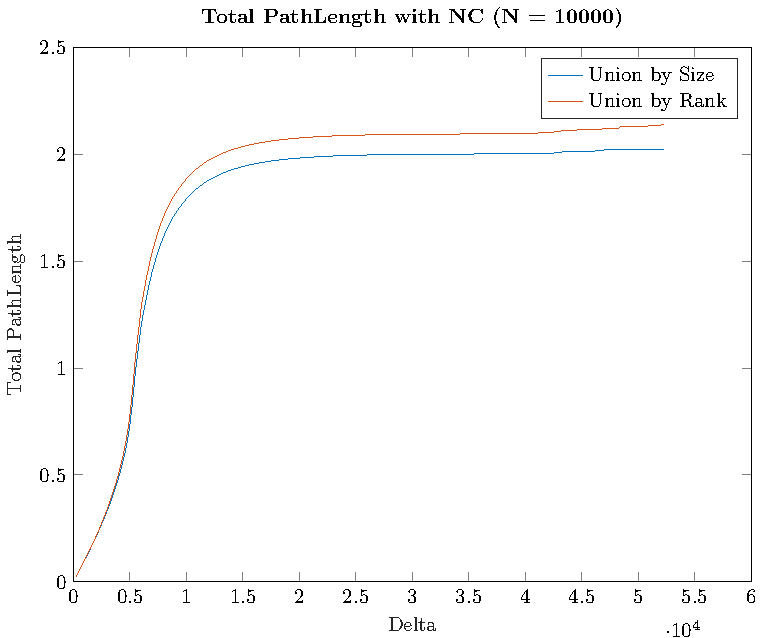
\includegraphics[width=\textwidth]{../images/plotNCNonFull10000_PathLength.pdf}
        \caption{Path Lengths with different union strategies with $n = 10000$ without Quick-Union}
    \end{subfigure}

    \caption{Total Path Length normalized with No Compression}
    \label{fig:tplNC}
\end{figure}
